% ViDBpedia — course-project report, NeurIPS preprint layout (same form as the group's earlier report).
% Compile with XeLaTeX (Overleaf: Menu > Compiler > XeLaTeX; the bundled latexmkrc selects it automatically)
% so that Vietnamese names such as "Trần Nhân Tông" are typeset correctly.
% In code listings, characters above U+00FF are wrapped in (*...*) escapes (listings + XeLaTeX limitation).
\documentclass{article}
\usepackage[preprint]{neurips_2024}
\makeatletter
\renewcommand{\@noticestring}{}   % no "Preprint" footer
\makeatother

\usepackage{amsmath}
\usepackage[math-style=TeX]{unicode-math}
% Times-like STIX Two for text and math (correct Vietnamese diacritics), Source Code Pro for code.
% Fonts are loaded by file name, which works on Overleaf (TeX Live) and with Tectonic.
\setmainfont{STIXTwoText}[Extension=.otf, UprightFont=*-Regular, BoldFont=*-Bold,
  ItalicFont=*-Italic, BoldItalicFont=*-BoldItalic]
\setmathfont{STIXTwoMath-Regular.otf}
\setsansfont{texgyreheros}[Extension=.otf, UprightFont=*-regular, BoldFont=*-bold,
  ItalicFont=*-italic, BoldItalicFont=*-bolditalic]
\setmonofont{SourceCodePro}[Extension=.otf, UprightFont=*-Regular, BoldFont=*-Bold, Scale=0.86]
\usepackage{graphicx}
\usepackage{booktabs}
\usepackage{array}
\newcolumntype{L}[1]{>{\raggedright\arraybackslash}p{#1}}
\usepackage{multirow}
\usepackage{xcolor}
\usepackage{url}
\usepackage{listings}
\usepackage{algorithm}
\usepackage{algpseudocode}
\usepackage{enumitem}
\usepackage{needspace}
\usepackage[hidelinks]{hyperref}
\setcitestyle{numbers,square}
\setlength{\textfloatsep}{12pt plus 2pt minus 4pt}
\setlength{\floatsep}{10pt plus 2pt minus 2pt}
\setlength{\intextsep}{10pt plus 2pt minus 2pt}

\definecolor{codebg}{HTML}{F7F7F9}
\definecolor{coderule}{HTML}{9A9A9A}
\definecolor{codekw}{HTML}{1F3FA8}
\definecolor{codecomment}{HTML}{2E7D32}
\definecolor{codestring}{HTML}{A31515}
\lstset{basicstyle=\ttfamily\scriptsize, columns=fullflexible, keepspaces=true, breaklines=true,
  frame=single, rulecolor=\color{coderule}, backgroundcolor=\color{codebg},
  numbers=left, numberstyle=\tiny\color{coderule}, numbersep=6pt, xleftmargin=14pt, framexleftmargin=12pt,
  aboveskip=4pt, belowskip=8pt, captionpos=t,
  keywordstyle=\color{codekw}, commentstyle=\color{codecomment}, stringstyle=\color{codestring},
  upquote=true, showstringspaces=false, escapeinside={(*}{*)}}
\lstdefinelanguage{sparql}{morekeywords={PREFIX,SELECT,CONSTRUCT,WHERE,FILTER,OPTIONAL,GROUP,BY,ORDER,BIND,AS,
  SERVICE,UNION,LIMIT,COUNT,DISTINCT,GROUP_CONCAT,EXISTS,NOT,IF,STR,LANG,STRSTARTS,VALUES},
  sensitive=true, morecomment=[l]{\#}, morestring=[b]"}
\lstdefinelanguage{turtle}{morekeywords={a,@prefix}, sensitive=true, morecomment=[l]{\#}, morestring=[b]"}
\lstdefinelanguage{yaml}{morecomment=[l]{\#}, morestring=[b]"}
\renewcommand{\lstlistingname}{Listing}
\newcommand{\cls}[1]{\ensuremath{\text{\textit{#1}}}}  % class / property name (text or math)
\newcommand{\ttl}[1]{\texttt{#1}}          % IRIs, code
\newcommand{\vidbo}{\ttl{vidbo}}

\title{ViDBpedia: An Inference-Rich Vietnamese\\DBpedia from Wikipedia Infoboxes}

\author{%
  Le Phu Tai\\ 20252268M\\ SoICT, HUST \And
  Nguyen Thi Mai Anh\\ 20252265M\\ SoICT, HUST \And
  Duong Hoang Hai\\ 20252273M\\ SoICT, HUST \And
  Le Van Luan\\ 20252572M\\ SoICT, HUST
}

\begin{document}

\maketitle

\begin{abstract}
Knowledge specific to Vietnam (its dynasties, mandarins, battles and the administrative map redrawn in 2025) is
thinly covered by DBpedia, and much of it is never written in any article. We build \textbf{ViDBpedia}, a Vietnamese
DBpedia, from the official Vietnamese Wikipedia dumps, and ask whether \emph{the ontology can make the knowledge graph
contain more than was extracted}. At its core is
\textbf{\vidbo}, an OWL~2~DL ontology of 48 classes and 115 properties designed from 18 competency questions: 13
defined classes classify entities by their relations (a monarch is a person who holds a reign), and 10 property chains
derive kinship, dynastic membership, geographic containment and war participation. A dump-based pipeline extracts
1.51M triples from 44{,}003 articles, and a generic OWL~2~RL reasoner plus six SPARQL rules materialises 2.64M more.
Our experiments show that (i)~all 18 competency questions are answered (median 44\,ms), each relying on inferred
triples; (ii)~the same axioms and SHACL shapes expose about 1{,}700 data-quality issues, including bugs in our own
extractor; (iii)~links to English DBpedia combine 32{,}136 verified interlanguage links with a Silk-style matcher of
96.4\% precision and 48.5\% recall; and (iv)~the HermiT tableau reasoner confirms our engine's inferences on a sample.
We also report where the approach fails, and publish the graph through a SPARQL endpoint, Linked Data pages and a
command-line client.
\end{abstract}

% =====================================================================
\section{Introduction}

\textbf{Motivation.} Wikipedia is written for people. The infobox of the Vietnamese article on Emperor Trần Nhân Tông
states that his father was Trần Thánh Tông, that he reigned from 1278 to 1293 and, in the article on the Battle of
Bạch Đằng, that he was one of its commanders. A machine cannot use any of this: it is wiki-text, not data. And even a
person reading the page cannot answer the simple question ``who was his paternal grandfather?'' without opening a
second article. DBpedia~\cite{auer2007dbpedia,lehmann2015dbpedia} solved the first half of this problem for English by
extracting infobox content into RDF and publishing it as Linked Data~\cite{bernerslee2006linked,heath2011linked};
language chapters such as the Greek edition~\cite{kontokostas2012greek} showed that local knowledge benefits from a
local extraction. Vietnamese Wikipedia has about 1.6 million articles, yet the English DBpedia contains few Vietnamese
dynasties, mandarins and battles, and nothing about the 2025 merger of provinces.

\textbf{Why it is hard.} Three properties make a Vietnamese DBpedia more than a copy of the English pipeline. First,
\textbf{heterogeneous input}: the same infobox appears under more than 100 template names, with Vietnamese and English
parameter names, and values such as ``14 tháng 4, năm 2021'', ``257 TCN'' (257~BCE) or ``4.412.264 người'' that no
off-the-shelf parser reads. Second, and more importantly, \textbf{implicit knowledge}: the answers to most interesting
questions are spread over several articles (a grandfather is in the father's article; a person born in a commune was
born within its province; a commander of a battle took part in the enclosing war). Third, \textbf{roles and change}:
monarch, mandarin and general are roles a person plays for a period, the royalty infobox is shared by monarchs,
consorts and heirs, and the administrative map changed in 2025, when Vietnam merged its provinces into 34 and
abolished the district level~\cite{resolution2025}.

\textbf{Our approach.} We follow the DBpedia architecture (dumps, mappings, extraction, linking, publication) but
put an expressive ontology at its centre and \emph{materialise} its consequences. Each competency question that the
graph should answer is turned into a SPARQL query, and axioms are added until the query is answered from the data:
defined classes for roles, property chains for multi-article relations, transitive and inverse properties for
hierarchies, reified tenures for time-bound roles, and explicit domain knowledge about the 2025 reform. The ontology
is used twice: during extraction, to reject triples whose types contradict a property's domain or range, and during
reasoning, to derive new triples and to detect contradictions.

\textbf{Contributions.}
\begin{enumerate}[leftmargin=*,itemsep=2pt]
  \item \textbf{\vidbo}, an OWL~2~DL ontology derived from 18 competency questions, whose defined classes, property
        chains, transitive and inverse properties infer kinship, dynastic membership, roles, geographic containment and
        war participation; it models reigns and offices as n-ary relations and encodes the 2025 administrative reform.
  \item A \textbf{reproducible dump-based extraction pipeline} with declarative infobox mappings, Vietnamese value
        parsers and a DBpedia-style ontology range check, producing 1.51M triples from 44{,}003 articles.
  \item A \textbf{generic OWL~2~RL forward-chaining reasoner} with a SPARQL rule layer that materialises 2.64M triples
        in 15 minutes on a laptop, cross-checked against the HermiT tableau reasoner.
  \item \textbf{Two-stage interlinking} with English DBpedia, evaluated against interlanguage links as a gold standard,
        and a SPARQL endpoint with dereferenceable Linked Data pages and a terminal client.
  \item An \textbf{analysis of failure cases}: where linking fails, how axioms act
        as a bug detector, and which of our own modelling decisions produced millions of wrong triples before we fixed them.
\end{enumerate}

% =====================================================================
\section{Related Work}

\textbf{DBpedia and its chapters.} DBpedia extracts Wikipedia dumps with a framework of extractors; the mapping-based
extractor turns infobox parameters into properties of the community-maintained DBpedia ontology, guided by a mappings
wiki~\cite{bizer2009dbpedia,lehmann2015dbpedia}. Internationalised chapters use IRIs in the local language and
interlanguage links to connect to the English edition~\cite{kontokostas2012greek}. Wikidata~\cite{vrandecic2014wikidata}
and YAGO~\cite{suchanek2007yago} are complementary knowledge graphs; YAGO in particular combines Wikipedia with a
taxonomy to type entities. Our work reuses the DBpedia architecture and naming conventions, but replaces the shallow
DBpedia ontology for our domain by a more expressive one and materialises its consequences.

\textbf{Linked Data and its quality.} The Linked Data principles and the 5-star scheme~\cite{bernerslee2006linked}
require data to be published in open, machine-readable formats, identified by dereferenceable URIs, queryable with W3C
standards such as SPARQL~1.1~\cite{sparql11}, and linked to other datasets. Knowledge-graph refinement and Linked Data
quality are surveyed in~\cite{paulheim2017refinement,zaveri2016quality}; we use two of the refinement strategies they
describe, axiom-based error detection and type inference, inside the construction pipeline rather than afterwards.

\textbf{Ontology engineering.} We follow Grüninger and Fox~\cite{gruninger1995methodology}: informal competency
questions (CQs) are formalised as queries and drive the choice of axioms. OntoClean~\cite{guarino2002ontoclean}
distinguishes rigid from non-rigid classes, which is why roles are defined rather than asserted in \vidbo, and
ontology design patterns~\cite{gangemi2005odp}, in particular the W3C n-ary relation pattern~\cite{noy2006nary},
guide the modelling of reigns and offices.

\textbf{Reasoning and validation.} OWL~2~\cite{owl2overview} offers several profiles~\cite{owl2profiles}; OWL~2~RL can
be implemented by forward-chaining rules and scales to large ABoxes, whereas tableau reasoners such as
HermiT~\cite{glimm2014hermit} decide full OWL~2~DL but do not scale to millions of assertions. We use both: an RL
engine on the full data and HermiT on a sample. SHACL~\cite{shacl2017} adds closed-world validation, complementing the
open-world semantics of OWL.

\textbf{Link discovery.} Silk~\cite{volz2009silk} specifies linkage rules that combine similarity metrics with
aggregations and thresholds. Our matcher implements such a rule (label similarity, type compatibility and dates) and
we also provide it as a Silk link specification.

% =====================================================================
\section{Problem Formulation, Data and Task}\label{sec:problem}

\textbf{Formulation.} Let $W$ be a set of Wikipedia articles and $\mathcal{O}$ an ontology. Extraction is a function
that maps each article to a set of RDF triples using a mapping $M$ from infobox parameters to ontology terms,
\begin{equation}
  \mathcal{A} \;=\; \bigcup_{w \in W} \mathrm{ext}_M(w) \;\subseteq\; I \times P \times (I \cup L),
\end{equation}
where $I$ is the set of resource IRIs, $P$ the properties and $L$ the literals. Reasoning computes the closure of the
extracted triples under the axioms of $\mathcal{O}$ and a set of rules $\mathcal{R}$; the inferred part is what the
ontology adds,
\begin{equation}
  \mathcal{A}^{*} = \mathrm{Cl}_{\mathcal{O},\mathcal{R}}(\mathcal{A}), \qquad
  \mathcal{A}_{\mathrm{inf}} = \mathcal{A}^{*} \setminus \mathcal{A}.
\end{equation}
Linking is a partial function $\ell : I \rightharpoonup I_{\mathrm{DBpedia}}$ published as \ttl{owl:sameAs}. The task is
judged by whether the competency questions, written as SPARQL queries $q_1,\dots,q_{18}$, return correct answers over
$\mathcal{A}^{*}$, by the size and correctness of $\mathcal{A}_{\mathrm{inf}}$, and by the precision and recall of $\ell$.

\textbf{Data.} We use the official Vietnamese Wikipedia dumps of 1~October~2026: the 1.16\,GB articles dump, the
language-link table and the page-properties table (Wikidata QIDs and disambiguation flags). A first pass over all
1{,}622{,}356 articles keeps those that use one of the mapped infobox templates or belong to seed categories such as
\emph{Vietnamese dynasties}, and records 317{,}604 redirects. A second pass adds pages linked from object-valued infobox
fields (parents, birth places, commanders), so that the objects of extracted triples are themselves described. The
result is 44{,}003 articles, 43{,}614 of which are not disambiguation pages. The most frequent infobox groups are
person (11{,}473 articles), officeholder (7{,}134), royalty (7{,}078), Vietnamese administrative unit (4{,}170),
military conflict (2{,}366), country or former state (1{,}754), settlement (1{,}446), military person (1{,}332), writer
(1{,}074), feudal-era official (560) and book (89). From them the extraction reads 209{,}775 object values (links),
70{,}865 literals, 43{,}873 dates and 11{,}205 numbers, and creates 20{,}755 office, 4{,}691 reign and 1{,}807
royal-title nodes.

\textbf{The task as competency questions.} The usage scenario is a user who queries Vietnamese history, geography and
notable people with SPARQL. We wrote 18 informal CQs before designing the ontology (Table~\ref{tab:cq} in
Section~\ref{sec:results}); examples are ``who is the paternal grandfather of Trần Nhân Tông?'', ``who was born within
today's Nghệ An province?'', ``which monarchs reigned while their dynasty was at war?'' and ``which districts were
abolished on 1~July~2025?''. None of them can be answered by a single infobox.

% =====================================================================
\section{Method}\label{sec:method}

Figure~\ref{fig:pipeline} summarises the pipeline. The ontology drives both the extraction (range check) and the
reasoning; one command rebuilds everything in about 1.5 hours on a laptop.

\begin{figure}[t]
  \centering
  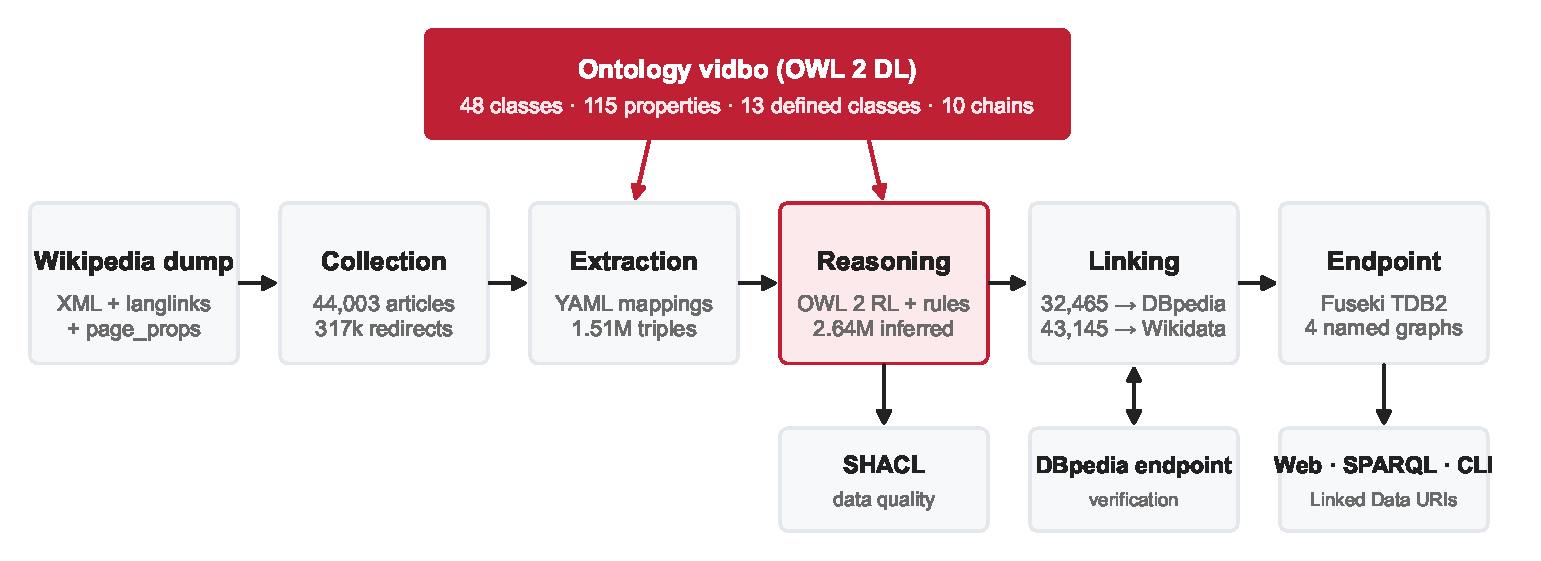
\includegraphics[width=0.8\textwidth]{figures/fig_pipeline.pdf}
  \caption{The ViDBpedia pipeline: dump collection, mapping-based extraction, OWL~2~RL reasoning with a rule layer,
  SHACL validation, linking to DBpedia and Wikidata, and publication on a Fuseki endpoint.}
  \label{fig:pipeline}
\end{figure}

\subsection{The \vidbo\ ontology}\label{sec:onto}

\textbf{From questions to terminology.} Terminology was grounded in the data: counting how often every infobox
parameter is used revealed, e.g., that 492 articles use the variant \ttl{Infobox officeholder 1} and 555 a dedicated
template for feudal-era officials.

\textbf{Class hierarchy.} Figure~\ref{fig:hier} shows the 48 classes under five top-level classes \cls{Agent},
\cls{Place}, \cls{Event}, \cls{Work} and \cls{Tenure}, aligned with DBpedia, FOAF and schema.org by 53 equivalence and
subsumption axioms, so that the graph can also be queried with those vocabularies. Disjointness axioms
($\cls{Person} \sqcap \cls{Place} \sqsubseteq \bot$, eight \texttt{AllDisjointClasses} groups in total) do not add facts
but expose contradictions. \cls{Group} (dynasties) is deliberately \emph{not} disjoint with \cls{Place}: Wikipedia uses
one article, e.g.\ ``Nhà Nguyên'', for both a ruling house and the polity it ruled.

\begin{figure}[t]
  \centering
  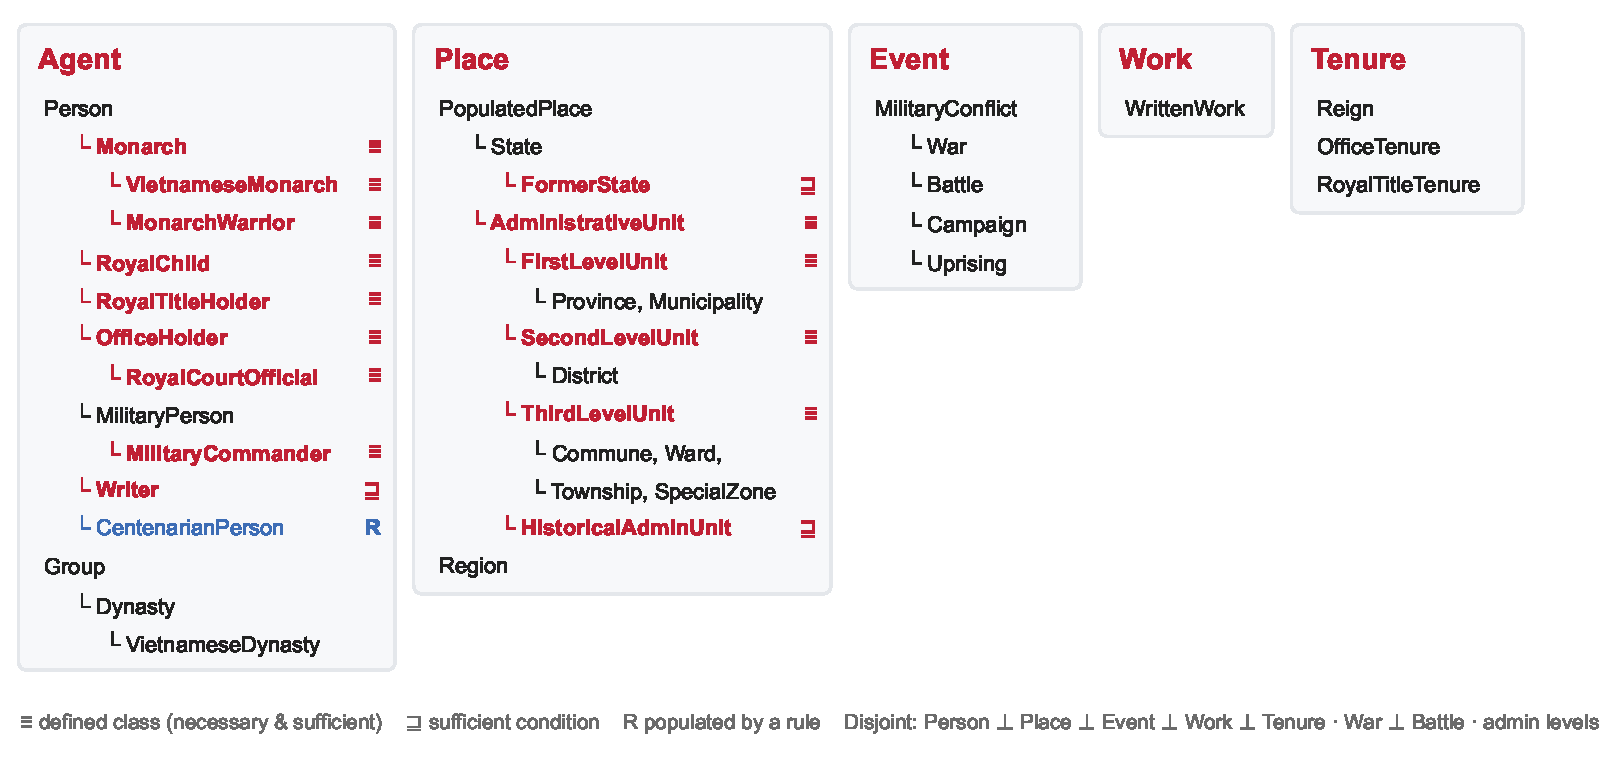
\includegraphics[width=0.72\textwidth]{figures/fig_hierarchy.pdf}
  \caption{Class hierarchy of \vidbo. Red classes are defined (membership is inferred by the reasoner); the blue class
  is populated by a SPARQL rule.}
  \label{fig:hier}
\end{figure}

\textbf{Roles as defined classes.} Being a monarch, an official or a commander is a \emph{role} that a person plays
for a period, not a rigid property of the person; OntoClean forbids placing such non-rigid classes as asserted
superclasses of rigid ones~\cite{guarino2002ontoclean}. We therefore never assert roles. Roles are \emph{defined}
through relations, and the reasoner classifies individuals; for instance
$\cls{Monarch} \equiv \cls{Person} \sqcap \exists \cls{hasReign}.\cls{Reign}$ and
$\cls{MonarchWarrior} \equiv \cls{Monarch} \sqcap \cls{MilitaryCommander}$. A single infobox line ``commander: Trần Nhân Tông'' on a battle page is therefore enough to classify him as a warrior
monarch. Table~\ref{tab:defined} lists the main defined classes with the number of members found on the full data.

\begin{table}[t]
  \caption{Selected defined classes and the number of members inferred on the full data.}
  \label{tab:defined}
  \centering\footnotesize
  \begin{tabular}{@{}l l r@{}}
    \toprule
    Class & Definition & Members\\
    \midrule
    \cls{Monarch} & $\cls{Person} \sqcap \exists\cls{hasReign}.\cls{Reign}$ & 3{,}981\\
    \cls{VietnameseMonarch} & $\cls{Monarch} \sqcap \exists\cls{memberOfDynasty}.\cls{VietnameseDynasty}$ & 169\\
    \cls{RoyalChild} & $\cls{Person} \sqcap \exists\cls{hasParent}.\cls{Monarch}$ & 6{,}160\\
    \cls{OfficeHolder} & $\cls{Person} \sqcap \exists\cls{holdsOffice}.\cls{OfficeTenure}$ & 6{,}832\\
    \cls{RoyalCourtOfficial} & $\cls{OfficeHolder} \sqcap \exists\cls{servedUnder}.\cls{Monarch}$ & 204\\
    \cls{MilitaryCommander} & $\cls{Person} \sqcap \exists\cls{commanded}.\cls{MilitaryConflict}$ & 10{,}257\\
    \cls{MonarchWarrior} & $\cls{Monarch} \sqcap \cls{MilitaryCommander}$ & 755\\
    \cls{ThirdLevelUnit} & $\cls{AdministrativeUnit} \sqcap \exists\cls{adminLevel}.\{3\}$ & 3{,}328\\
    \bottomrule
  \end{tabular}
\end{table}

\textbf{Property axioms.} Ten property chains derive relations that are never written in Wikipedia, for example
\begin{align}
  \cls{hasFather} \circ \cls{hasFather} &\equiv \cls{hasPaternalGrandfather}, \\
  \cls{hasFather} \circ \cls{memberOfDynasty} &\sqsubseteq \cls{memberOfDynasty}, \\
  \cls{bornWithin} \circ \cls{locatedIn} &\sqsubseteq \cls{bornWithin}, \\
  \cls{participatedIn} \circ \cls{partOfConflict} &\sqsubseteq \cls{participatedIn}.
\end{align}
The chain on \cls{memberOfDynasty} encodes patrilineal dynastic membership; the chains on \cls{bornWithin} and
\cls{participatedIn} are right-recursive and, together with
$\cls{birthPlace} \sqsubseteq \cls{bornWithin}$ and $\cls{commanded} \sqsubseteq \cls{participatedIn}$, answer ``who was
born in today's Nghệ An province'' when an infobox only names a district, and ``who took part in the Mongol--Đại Việt
war'' when an infobox only names a battle. Seven properties are transitive (\cls{locatedIn}, \cls{partOfConflict},
\cls{hasAncestor}, \cls{intellectualLineage}, \ldots), 18 pairs of properties are declared inverse, \cls{spouse} and
\cls{sibling} are symmetric and irreflexive, \cls{hasParent} is irreflexive and asymmetric, and \cls{hasFather},
\cls{birthDate} and \cls{adminLevel} are functional. Relations that OWL cannot express are delegated to the rule layer
(Section~\ref{sec:reason}): \cls{sibling} requires $x \neq y$, and its result feeds the chain
$\cls{uncleOrAunt} \equiv \cls{hasParent} \circ \cls{sibling}$. Table~\ref{tab:props} gives an overview of the object
properties grouped by sub-domain.

\begin{table}[t]
  \caption{Main object properties of \vidbo\ and their characteristics (T = transitive, S = symmetric,
  I = irreflexive, A = asymmetric, F = functional, IF = inverse functional).}
  \label{tab:props}
  \centering\footnotesize
  \setlength{\tabcolsep}{3.5pt}
  \begin{tabular}{@{}l L{3.3cm} L{2.2cm} c L{5.2cm}@{}}
    \toprule
    Group & Property & Domain $\to$ range & Char. & Axioms / role in inference\\
    \midrule
    \multirow{6}{*}{Family}
      & \cls{hasParent} & Person $\to$ Person & I, A & $\sqsubseteq \cls{hasAncestor}$; $\equiv \cls{hasChild}^-$\\
      & \cls{hasFather}, \cls{hasMother} & Person $\to$ Person & F & $\sqsubseteq \cls{hasParent}$; $\equiv$ \ttl{dbo:father}/\ttl{dbo:mother}\\
      & \cls{hasAncestor} & -- & T & $\equiv \cls{hasDescendant}^-$\\
      & \cls{hasGrandparent}, \cls{hasPaternalGrandfather} & -- & -- & chains $\cls{hasParent}\circ\cls{hasParent}$, $\cls{hasFather}\circ\cls{hasFather}$\\
      & \cls{spouse}, \cls{sibling} & Person $\to$ Person & S, I & \cls{sibling} materialised by rule R1\\
      & \cls{uncleOrAunt} & -- & -- & chain $\cls{hasParent}\circ\cls{sibling}$\\
    \midrule
    \multirow{4}{*}{\shortstack[l]{Dynasty,\\office}}
      & \cls{memberOfDynasty} & Person $\to$ Dynasty & -- & chains $\cls{hasFather}\circ\cls{memberOfDynasty}$, $\cls{hasReign}\circ\cls{tenureDynasty}$\\
      & \cls{hasReign}, \cls{holdsOffice}, \cls{holdsRoyalTitle} & Person $\to$ Tenure & IF & n-ary relations; define \cls{Monarch}, \cls{OfficeHolder}, \cls{RoyalTitleHolder}\\
      & \cls{servedUnder} & -- & -- & chain $\cls{holdsOffice}\circ\cls{underMonarch}$; defines \cls{RoyalCourtOfficial}\\
      & \cls{predecessor}, \cls{successor} & Person $\to$ Person & I & inverse pair; deliberately not transitive\\
    \midrule
    \multirow{4}{*}{Geography}
      & \cls{locatedIn} & Place $\to$ Place & T & $\equiv \cls{contains}^-$; $\sqsubseteq$ \ttl{dbo:isPartOf}\\
      & \cls{province}, \cls{district}, \cls{region} & -- $\to$ admin.\ unit & -- & $\sqsubseteq \cls{locatedIn}$\\
      & \cls{seatOf} & Place $\to$ Place & -- & $\sqsubseteq \cls{locatedIn}$, $\sqsubseteq \cls{capitalOf}$; $\equiv \cls{adminSeat}^-$\\
      & \cls{bornWithin}, \cls{diedWithin} & -- & -- & $\cls{birthPlace} \sqsubseteq \cls{bornWithin}$; chain with \cls{locatedIn}\\
    \midrule
    \multirow{4}{*}{Military}
      & \cls{commander} & Conflict $\to$ Person & -- & $\equiv \cls{commanded}^-$; $\cls{commanded} \sqsubseteq \cls{participatedIn}$\\
      & \cls{partOfConflict} & Conflict $\to$ Conflict & T & $\equiv \cls{hasSubConflict}^-$\\
      & \cls{participatedIn} & Person $\to$ Conflict & -- & chain $\cls{participatedIn}\circ\cls{partOfConflict}$\\
      & \cls{conflictPlace} & Conflict $\to$ Place & -- & $\sqsubseteq \cls{tookPlaceWithin}$; chain with \cls{locatedIn}\\
    \midrule
    \multirow{2}{*}{Works}
      & \cls{notableWork} & Person $\to$ Work & -- & $\equiv \cls{author}^-$; $\exists\cls{notableWork}.\cls{WrittenWork} \sqsubseteq \cls{Writer}$\\
      & \cls{influencedBy} & Person $\to$ Person & I & $\equiv \cls{influenced}^-$; $\sqsubseteq \cls{intellectualLineage}$ (T)\\
    \bottomrule
  \end{tabular}
\end{table}

\textbf{N-ary relations.} ``Trần Nhân Tông reigned as Emperor of Đại Việt for the Trần dynasty from 8~November~1278 to
16~April~1293'' has five arguments, so following the W3C pattern~\cite{noy2006nary} it becomes a \cls{Reign} node
that carries the title, the dynasty and the dates; \cls{OfficeTenure} and \cls{RoyalTitleTenure} are analogous. The
royalty infobox is shared by monarchs, consorts and heirs, all of whom have a ``reign'' field; titles such as
\emph{hoàng hậu} (empress consort) are mapped to \cls{RoyalTitleTenure}, which is disjoint from \cls{Reign}, otherwise
consorts would be classified as monarchs. The chain $\cls{hasReign} \circ \cls{tenureDynasty} \sqsubseteq
\cls{memberOfDynasty}$ connects a monarch to the dynasty recorded on the reign.

\textbf{The 2025 administrative reform.} Administrative levels are defined by value restrictions
($\cls{FirstLevelUnit} \equiv \cls{AdministrativeUnit} \sqcap \exists \cls{adminLevel}.\{1\}$), the domain knowledge
$\cls{SecondLevelUnit} \sqsubseteq \cls{HistoricalAdministrativeUnit}$ records that districts were abolished on
1~July~2025, and administrative units have the key \cls{adminCode}. A key is an OWL~2 feature that would, under OWL
semantics, make two units with the same code the same individual; we use it to \emph{report} reused codes instead
(Section~\ref{sec:quality}).

\textbf{OWL~2~DL compliance.} \texttt{xsd:date} and \texttt{xsd:gYear} are not in the OWL~2 datatype map, and HermiT
rejects ontologies that use them as ranges. We keep these datatypes in the data, exactly like DBpedia, record the
expected datatype with an annotation property, and enforce it with SHACL.

\subsection{Mapping-based extraction}\label{sec:extract}

\textbf{Collection from dumps.} The MediaWiki API throttles anonymous clients to roughly 50 pages per minute, which
would take about eight hours for our scope; like the DBpedia extraction framework we therefore stream the dumps
(Section~\ref{sec:problem}). Infoboxes are parsed with \ttl{mwparserfromhell}.

\textbf{Declarative mappings.} A YAML file plays the role of the DBpedia mappings wiki: 11 template groups map
Vietnamese and English parameter names to \vidbo\ properties, and numbered parameter groups (``\emph{tại vị} 2'',
\ttl{office3}) become tenure nodes. Listing~\ref{lst:mapping} shows an excerpt; the triples it produces for one
article are shown, together with what the reasoner adds, in Listing~\ref{lst:sample}.

\begin{lstlisting}[language=yaml, caption={Excerpt of the royalty mapping. Each parameter accepts its Vietnamese and English names.}, label=lst:mapping]
royalty:
  names: [Thông tin nhân v(*ậ*)t hoàng gia, Infobox royalty, ...]
  class: Person
  properties:
    "cha|father": {prop: hasFather, kind: object, max: 1}
    "sinh|birth_date": {prop: birthDate, kind: date, year_prop: birthYear}
    "mi(*ế*)u hi(*ệ*)u|temple name": {prop: templeName, kind: literal}
  tenure:                       # numbered groups -> one Reign node each
    class: Reign
    link: hasReign
    fields:
      "ch(*ứ*)c v(*ị*)|succession": {prop: position, kind: literal}
      "t(*ạ*)i v(*ị*)|reign": {kind: period}
      "ti(*ề*)n nhi(*ệ*)m|predecessor": {prop: predecessor, kind: object, attach: person}
\end{lstlisting}


\textbf{Vietnamese value parsers.} Dates appear as ``14 tháng 4, năm 2021'', as templates such as
\ttl{\{\{ngày sinh|1766|1|3\}\}} or \ttl{\{\{birth date|1258|12|7\}\}}, and as years BCE written ``257 TCN''; periods
appear as ``[[8 tháng 11]] năm [[1278]] -- [[16 tháng 4]] năm [[1293]]''; numbers use Vietnamese formatting
(``4.412.264'', ``3.942,62\,km²''); and lists hide links inside templates such as \ttl{\{\{plain list\}\}}. The parsers
are covered by 16 unit tests. One early bug illustrates why the tests matter: in ``14 tháng 4, năm 2021'' the first
version took the day as the year.

\textbf{IRIs and provenance.} Resource IRIs follow the article titles (\ttl{vidbr:Trần\_Nhân\_Tông}), links to
redirects are resolved to canonical IRIs, and every resource records its page ID and revision as provenance.

\textbf{Ontology range check.} Following DBpedia, an object triple whose subject or object has an asserted class
disjoint with the property's domain or range (taking super-properties and inverse properties into account) is moved
into a separate dataset instead of the main graph. It removed 536 triples such as ``the predecessor of Lý Thái Tổ is the
Đinh dynasty'' (a dynasty, not a person). Table~\ref{tab:datasets} lists the resulting datasets, named as in DBpedia.

\begin{table}[t]
  \caption{Extracted datasets. A twelfth dataset holds the 536 triples removed by the range check.}
  \label{tab:datasets}
  \centering\footnotesize
  \begin{tabular}{@{}l r l@{}}
    \toprule
    Dataset & Triples & Content\\
    \midrule
    article\_categories & 353{,}687 & \ttl{dct:subject}, SKOS categories\\
    page\_metadata & 256{,}546 & page ID, revision, provenance\\
    mappingbased\_literals & 239{,}831 & dates, numbers, codes, names\\
    mappingbased\_objects & 206{,}184 & entity--entity relations\\
    tenures & 135{,}405 & reified reigns, offices and royal titles\\
    abstracts & 87{,}172 & first paragraph of the article\\
    wikidata\_links & 86{,}290 & \ttl{owl:sameAs} to Wikidata\\
    instance\_types & 45{,}575 & types from template, title and category\\
    labels & 43{,}614 & \ttl{rdfs:label}@vi\\
    redirects & 43{,}140 & \ttl{wikiPageRedirects}\\
    geo\_coordinates & 13{,}745 & WGS84 latitude and longitude\\
    \midrule
    Total & 1{,}511{,}189 & \\
    \bottomrule
  \end{tabular}
\end{table}

\subsection{Reasoning}\label{sec:reason}

\textbf{Why materialise.} Materialising inferences lets the SPARQL endpoint answer CQs without query-time reasoning,
and makes every inferred triple inspectable. Off-the-shelf pure-Python OWL~RL engines were too slow for 1.5M triples,
so we implemented a generic forward-chaining reasoner that reads the axioms of \vidbo\ and applies the OWL~2~RL/RDF
rules~\cite{owl2profiles} for class and property hierarchies, equivalence, intersection and union,
\texttt{someValuesFrom} and \texttt{hasValue} restrictions, domain and range, inverse, symmetric and transitive
properties and property chains (\texttt{cax-sco}, \texttt{cls-int1/2}, \texttt{cls-svf1}, \texttt{cls-hv1/2},
\texttt{prp-dom}, \texttt{prp-rng}, \texttt{prp-inv1/2}, \texttt{prp-symp}, \texttt{prp-trp}, \texttt{prp-spo1/2})
until a fix-point is reached. Nothing about the domain is hard-coded: changing the ontology changes the result.

\textbf{Consistency rules are reported, not applied.} The rules \texttt{cax-dw}, \texttt{prp-irp}, \texttt{prp-asyp},
the functional-property rules and \texttt{prp-key} would derive \texttt{owl:sameAs} or inconsistency. We \emph{report}
their violations instead: applying \texttt{prp-key}, for instance, would merge a new commune with the dissolved commune
whose code it reuses.

\textbf{Engine.} Algorithm~\ref{alg:reason} outlines the engine. The TBox is compiled once into lookup tables
(super-class and super-property closures, inverse pairs, chains, restrictions); the ABox is held as one set of
subject--object pairs per property and one set of types per individual, so that each rule is a set operation.
Transitive closure is computed per property by a graph search from every node, and a two-step chain
$p_1 \circ p_2 \sqsubseteq p$ is a hash join of $p_1$ with $p_2$ indexed by subject. Rounds are naive (every rule is applied to all facts), which is simple and sufficient here: 97\% of
the new triples appear in the first two rounds and the remaining rounds add only the tails of long chains. Starting
from 626{,}995 core triples (labels, categories and metadata do not take part), the fix-point is reached after
26 rounds, about 15 minutes, with 2{,}636{,}065 inferred triples.

\begin{algorithm}[t]
\caption{Materialisation (OWL~2~RL rules + rule layer)}
\label{alg:reason}
\small
\begin{algorithmic}[1]
\Require ontology $\mathcal{T}$, extracted triples $\mathcal{A}$, SPARQL rules $\mathcal{R}$
\State compile $\mathcal{T}$: $\mathit{sup}^*(C)$, $\mathit{supP}^*(p)$, inverses, chains, $\exists$/$\ni$ restrictions, intersections
\Procedure{Closure}{$\mathcal{A}$}
  \Repeat
    \State add $(s,o)$ to $q$ for every $q \in \mathit{supP}^*(p)$ \Comment{prp-spo1, prp-eqp}
    \State add $(o,s)$ to $p^-$; add $(o,s)$ to $p$ if $p$ is symmetric \Comment{prp-inv, prp-symp}
    \State replace $p$ by its transitive closure if $p$ is transitive \Comment{prp-trp}
    \State add $p_1 \bowtie p_2$ to $p$ for each chain $p_1\circ p_2 \sqsubseteq p$ \Comment{prp-spo2}
    \State type subjects and objects by domains and ranges \Comment{prp-dom, prp-rng}
    \State apply $\exists p.C$ and $\exists p.\{v\}$ restrictions \Comment{cls-svf1, cls-hv1/2}
    \State add $\mathit{sup}^*(C)$ to every type set; add intersections \Comment{cax-sco, cls-int1/2}
  \Until{no new triple}
\EndProcedure
\State \Call{Closure}{$\mathcal{A}$};\; $\mathcal{A} \gets \mathcal{A} \cup \mathcal{R}(\mathcal{A})$;\; \Call{Closure}{$\mathcal{A}$}
\State report disjointness, irreflexivity, asymmetry, functionality, key and cycle violations
\end{algorithmic}
\end{algorithm}

\textbf{Rule layer.} Six SPARQL \texttt{CONSTRUCT} rules cover what OWL cannot express (Table~\ref{tab:rules}): a
different-individual condition, arithmetic and comparisons of dates. The OWL closure is computed again after the rules,
so their results feed the axioms: the sibling rule R1, for instance, feeds the chain for uncles and aunts. Because the
rules are plain SPARQL (Listing~\ref{lst:rules}), any SPARQL engine can execute them.

\begin{table}[t]
  \caption{Rule layer (SPARQL \texttt{CONSTRUCT}) and the number of triples each rule derives.}
  \label{tab:rules}
  \centering\footnotesize
  \begin{tabular}{@{}l l r@{}}
    \toprule
    Rule & Derives & Triples\\
    \midrule
    R1 & \cls{sibling}: two different persons sharing a parent ($x \neq y$) & 54{,}710\\
    R2 & \cls{ageAtDeath} from birth and death years & 10{,}936\\
    R3 & \cls{CentenarianPerson} (age at death $\geq 100$) & 127\\
    R4 & \cls{durationYears} of reigns and offices & 22{,}090\\
    R5 & \cls{populationDensity} of administrative units & 5{,}421\\
    R6 & \cls{reignedDuringConflict}: reign overlaps a war of the monarch's dynasty & 670\\
    \bottomrule
  \end{tabular}
\end{table}

\begin{lstlisting}[language=sparql, caption={Two rules of the rule layer: the sibling rule and the temporal rule R6.}, label=lst:rules]
# R1 - siblings: two DIFFERENT persons sharing a parent
CONSTRUCT { ?x vidbo:sibling ?y }
WHERE { ?x vidbo:hasParent ?p . ?y vidbo:hasParent ?p . FILTER (?x != ?y) }

# R6 - a monarch reigned during a conflict fought by his dynasty
CONSTRUCT { ?m vidbo:reignedDuringConflict ?c }
WHERE {
  ?m vidbo:hasReign ?r ; vidbo:memberOfDynasty ?dyn .
  ?r vidbo:startYear ?rs ; vidbo:endYear ?re .
  ?c vidbo:combatant ?dyn ; vidbo:startYear ?cs .
  FILTER (xsd:integer(STR(?rs)) <= xsd:integer(STR(?cs)) &&
          xsd:integer(STR(?cs)) <= xsd:integer(STR(?re))) }
\end{lstlisting}

\subsection{Validation}\label{sec:validate}

OWL makes the open-world assumption: a missing value is unknown, not wrong. A qualified cardinality restriction such
as ``a military conflict has at least two combatants'' therefore never reports a conflict with one combatant listed.
SHACL~\cite{shacl2017} shapes encode the closed-world constraints we need: required labels, at most one birth date,
the pattern of administrative codes (2, 3 or 5 digits), coordinate ranges and the order of start and end years.
Because \texttt{sh:lessThanOrEquals} is undefined for \texttt{xsd:gYear} (including negative, BCE years), year order is
checked by a SHACL-SPARQL constraint that compares integer casts (Listing~\ref{lst:shacl}). Validation runs over the
extracted and inferred triples restricted to the 18 predicates the shapes inspect, about one million triples.

\begin{lstlisting}[language=turtle, caption={SHACL-SPARQL constraint checking that end years do not precede start years.}, label=lst:shacl]
vidbo:YearOrderConstraint a sh:SPARQLConstraint ;
  sh:select """SELECT $this ?start ?end WHERE {
      { $this vidbo:birthYear ?start ; vidbo:deathYear ?end }
      UNION { $this vidbo:startYear ?start ; vidbo:endYear ?end }
      FILTER (xsd:integer(STR(?end)) < xsd:integer(STR(?start))) }""" .
\end{lstlisting}

\subsection{Interlinking with English DBpedia}\label{sec:link}

\textbf{Stage 1: verified interlanguage links.} The dumps contain 33{,}278 Vietnamese-to-English language links for
our 43{,}614 non-disambiguation articles. A language link names an English \emph{article}, which is not necessarily a
DBpedia \emph{resource}: the article may be newer than the DBpedia release or may have been renamed. Each candidate
\ttl{dbr:} IRI is therefore verified against the public DBpedia endpoint and DBpedia redirects are followed.

\textbf{Stage 2: a Silk-style matcher.} The 10{,}930 entities without a language link are matched with a linkage rule.
Candidates are retrieved by exact label lookup on label variants (the original title, the title without diacritics,
and type-specific variants such as ``Battle of \ldots'', ``\ldots{} dynasty'' and ``\ldots{} province''). Each
candidate $c$ of an entity $e$ receives the score
\begin{equation}
  s(e,c) = 0.55\, \mathrm{JW}\big(\mathrm{fold}(l_e), \mathrm{fold}(l_c)\big) + 0.25\, \tau(e,c) + 0.20\, \upsilon(e,c),
\end{equation}
where $\mathrm{JW}$ is the Jaro--Winkler similarity of the labels after removing diacritics and parenthesised
qualifiers, $\tau \in \{0.5, 1\}$ rewards compatible types between \vidbo\ and DBpedia classes, and $\upsilon$ rewards
agreement of birth or start years ($1$ for equal years, $0.7$ within two years, $0.2$ otherwise, $0.6$ if unknown).
Two vetoes set $s = 0$: incompatible types, and a difference of more than two years in the birth year of a person. A
candidate is accepted if $s \geq 0.88$ and sent to manual review if $0.75 \leq s < 0.88$. The same rule is provided as
a Silk link specification, and the scoring function is a dozen lines of Python in \ttl{src/link.py}.

\textbf{Engineering for an unreliable endpoint.} The public endpoint was unavailable several times, so the linker
caches every answer and re-asks only missing queries on the next run. The current DBpedia release no longer publishes
\ttl{dbo:wikiPageID} or \ttl{dbo:abstract}, so existence is tested with \ttl{rdfs:label}. Links to Wikidata come from
the QIDs in the page-properties table.

\subsection{Publication}\label{sec:pub}

The graph is loaded into an Apache Jena Fuseki~\cite{jena} TDB2 store with four named graphs, \emph{ontology},
\emph{data}, \emph{inferred} and \emph{links}, whose union is the default graph, so that any triple can be traced to its
origin. A web front end (Figure~\ref{fig:ui}) offers DBpedia-style resource pages that badge every value as extracted,
inferred or linked, a SPARQL editor preloaded with the 18 CQs, an ontology browser and a label search. Resource URIs
are dereferenceable: \ttl{/resource/X} answers with HTTP~303 to an HTML page or, by content negotiation, to Turtle,
RDF/XML or JSON-LD. A terminal client runs ad-hoc queries, query files or numbered CQs. Together with the CC~BY-SA
licence inherited from Wikipedia and the links to DBpedia and Wikidata, this meets all five Linked Data stars.

\begin{figure}[t]
  \centering
  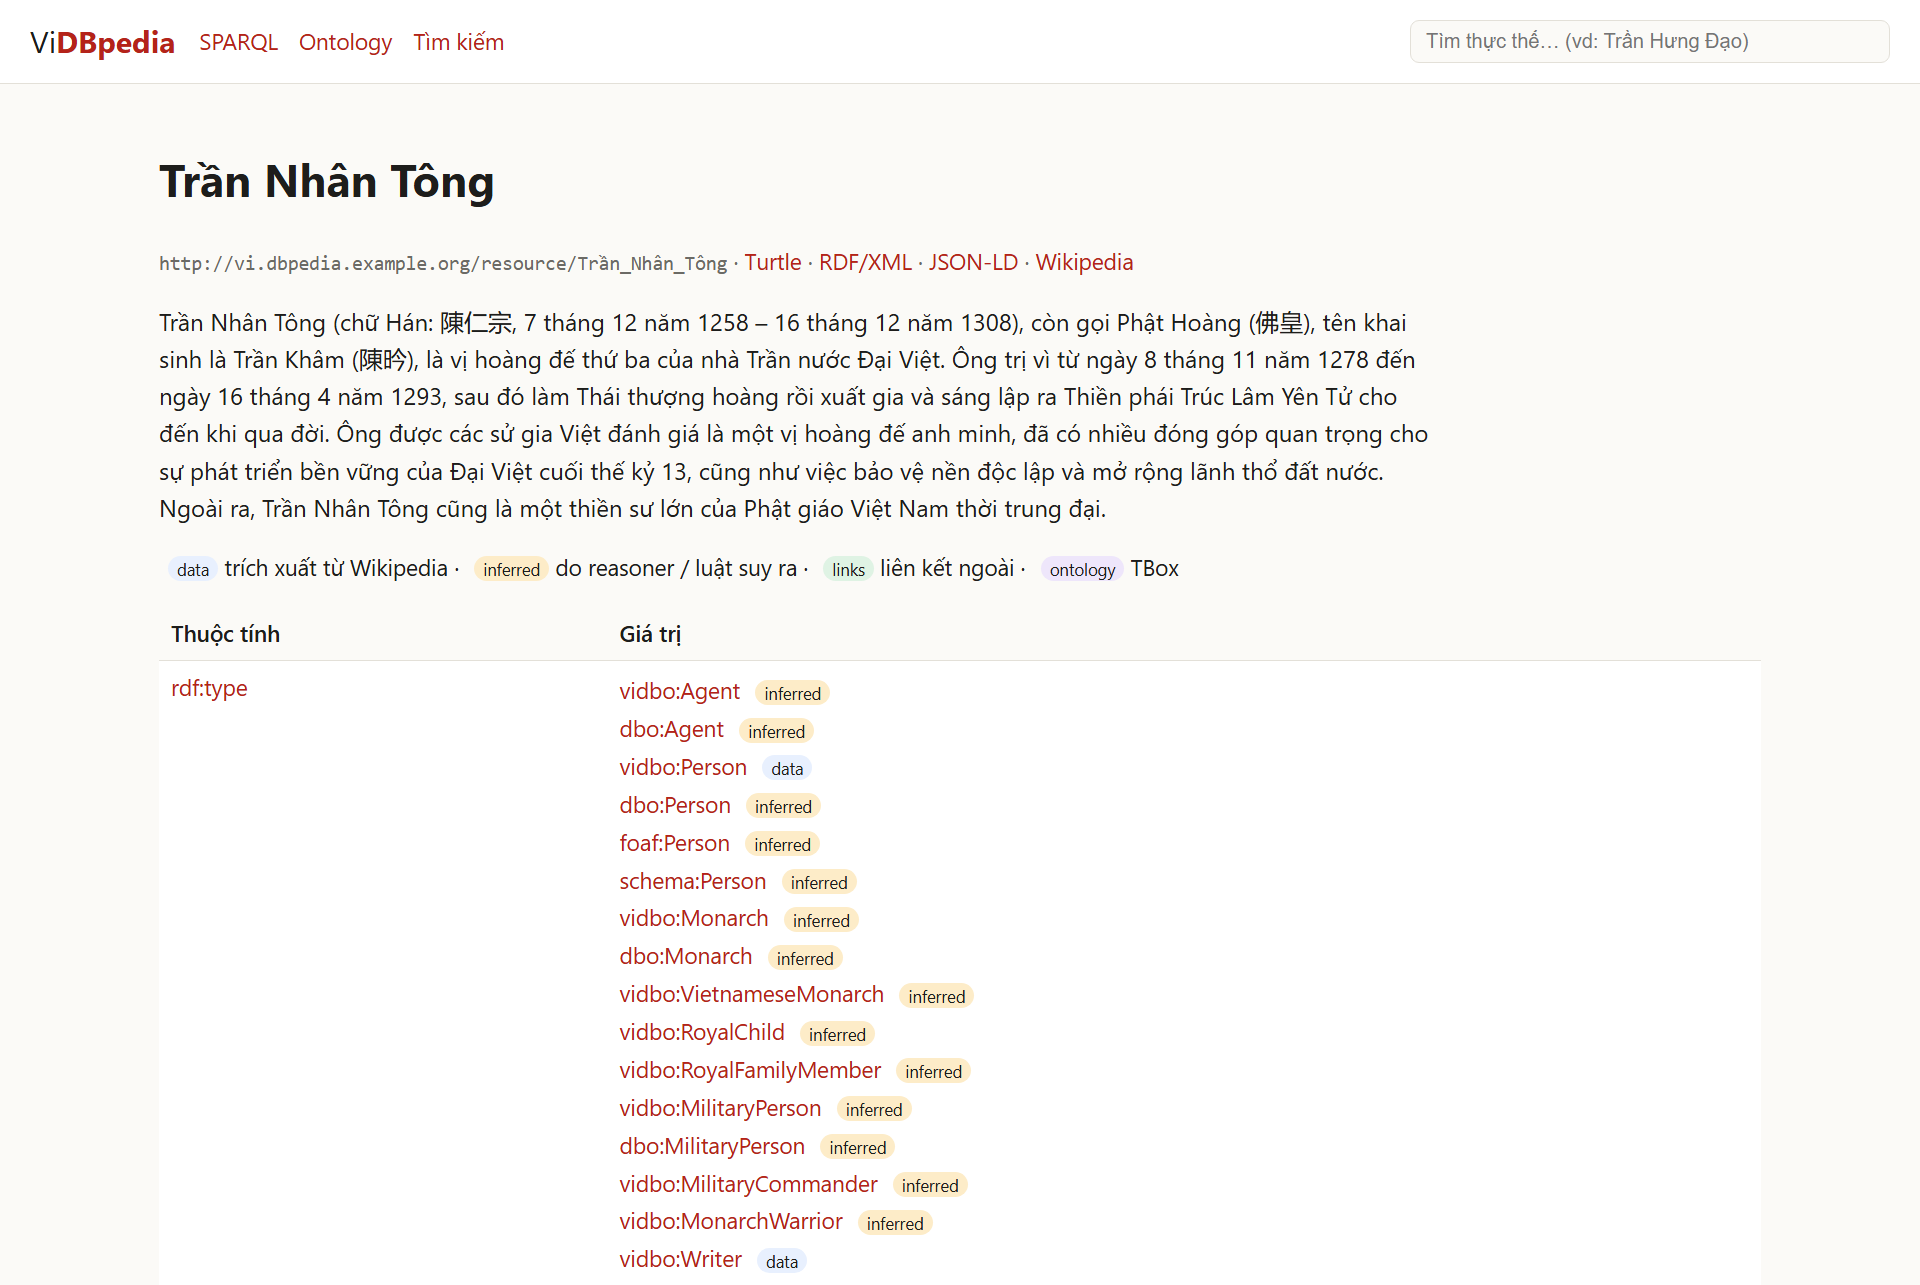
\includegraphics[width=0.49\textwidth]{figures/web_page.png}\hfill
  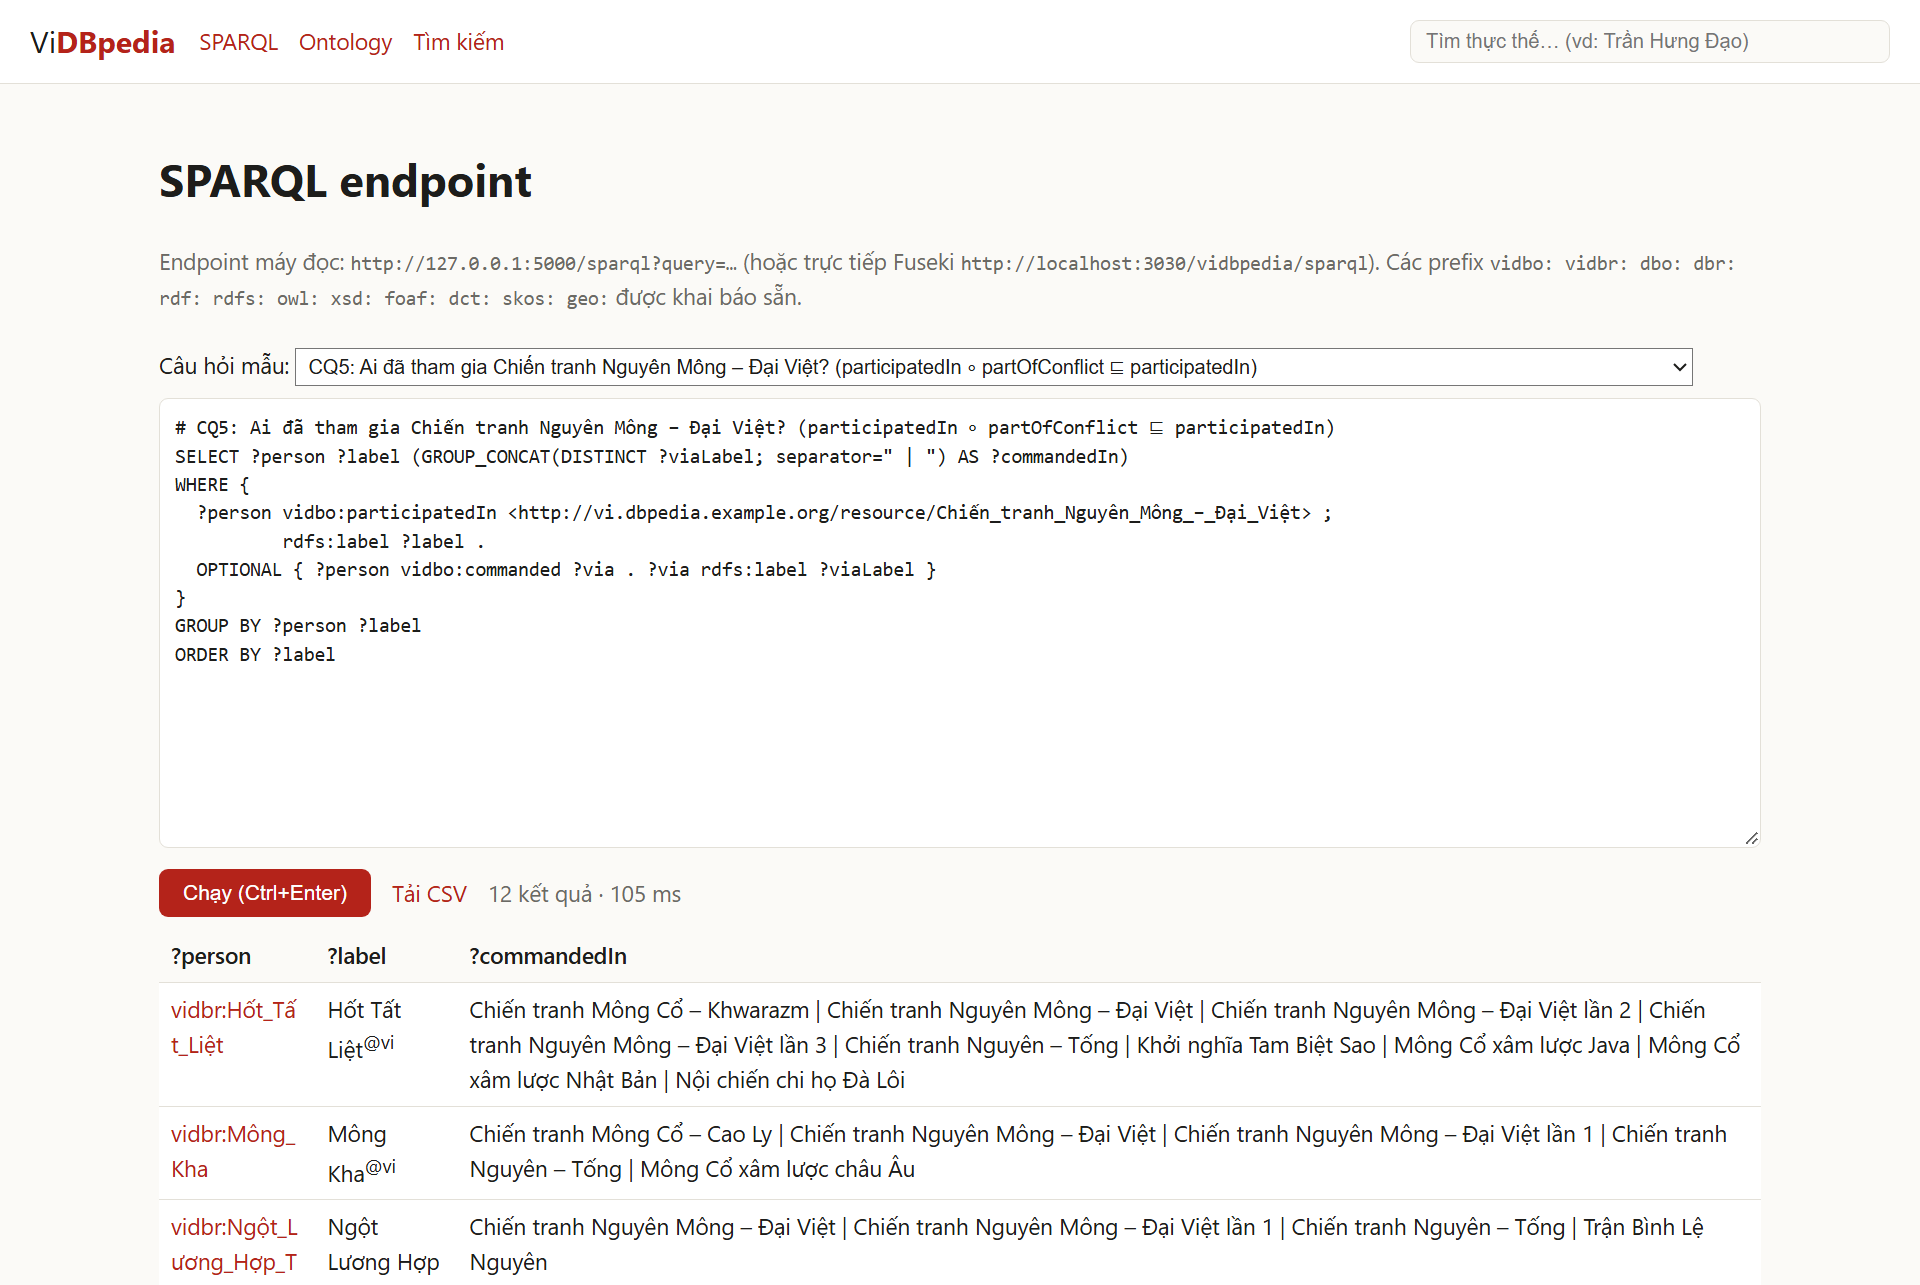
\includegraphics[width=0.49\textwidth]{figures/web_sparql.png}
  \caption{Left: resource page of Trần Nhân Tông, with \emph{data} and \emph{inferred} badges. Right: the SPARQL
  editor answering CQ5 in 105\,ms.}
  \label{fig:ui}
\end{figure}

% =====================================================================
\section{Experimental Setup}\label{sec:setup}

\textbf{Protocol.} All steps run on one Windows laptop with 16\,GB of RAM, Python~3.13 and Java for Fuseki~5.6.0; the
public DBpedia endpoint is the only external service. Table~\ref{tab:runtime} lists the steps and their run time. Each
step reads the output of the previous one from disk, so any step can be re-run alone. Validation is the slowest step,
most of it spent in the per-node SPARQL constraint of pySHACL; reasoning keeps the whole ABox in memory as Python sets.

\begin{table}[t]
  \caption{Pipeline steps, outputs and run time on a laptop.}
  \label{tab:runtime}
  \centering\footnotesize
  \begin{tabular}{@{}l l r@{}}
    \toprule
    Step (script) & Output & Time\\
    \midrule
    \ttl{collect\_dump.py} & 44{,}003 articles, 317{,}604 redirects & 13 min\\
    \ttl{extract.py} & 12 datasets, 1.51M triples & 10 min\\
    \ttl{reason.py} & 2.64M inferred triples, consistency report & 15 min\\
    \ttl{validate.py} & SHACL report (104 violations) & 17 min\\
    \ttl{link.py} & 32{,}465 DBpedia links, linking evaluation & 30--60 min\textsuperscript{a}\\
    \ttl{load\_endpoint.py} & Fuseki TDB2 store, 4 named graphs & 1 min\\
    \bottomrule
    \multicolumn{3}{@{}l}{\footnotesize \textsuperscript{a}depends on the availability of the public DBpedia endpoint; answers are cached}
  \end{tabular}
\end{table}

\textbf{Competency questions.} Each of the 18 CQs is a SPARQL file run against the local endpoint by
\ttl{src/run\_cqs.py}, which records the number of rows and the execution time and writes the results to a report. A
CQ counts as answered if it returns a non-empty result that we checked by hand against Wikipedia. For each CQ we also
record which axioms or rules make it answerable.

\textbf{Linking gold set and metrics.} Stage~2 is evaluated on entities whose true link is known: we sample 1{,}500
entities that \emph{do} have a verified language link, hide that link, and run the matcher. Let TP be the accepted
candidates equal to the true link, FP the accepted candidates that differ from it, and $n$ the sample size. We report
\begin{equation}
  P = \frac{\mathrm{TP}}{\mathrm{TP} + \mathrm{FP}}, \qquad R = \frac{\mathrm{TP}}{n}, \qquad
  F_1 = \frac{2PR}{P + R},
\end{equation}
overall and per class. Recall is measured against all sampled entities, so an entity for which the matcher finds no
candidate counts as a miss.

\textbf{Reproducibility.} All code, mappings, rules and queries are in the project repository. After downloading the three dump files,
\ttl{python run\_pipeline.py} runs every step of Table~\ref{tab:runtime} (\ttl{--from reason} or \ttl{--skip link}
restart or skip steps), and \ttl{python src/serve.py} starts Fuseki and the web interface. Two automated tests accompany
the code: \ttl{tests/test\_parsers.py} (16 cases for dates, periods, numbers and links) and \ttl{tests/test\_hermit.py}
(HermiT on the Trần sample). \ttl{src/run\_cqs.py} re-runs the 18 competency questions and writes their results to a
report.

% =====================================================================
\section{Results and Analysis}\label{sec:results}

\subsection{Inference yield}

By mechanism, the 2.64M inferred triples come from transitive closure (1{,}318k), alignment with the DBpedia, FOAF
and schema.org vocabularies (626k), class membership (276k), property chains (230k), the SPARQL rules (94k) and
inverse and sub-properties (91k); Table~\ref{tab:toppred} lists the properties that gain the most. Transitive closure
dominates in volume, mostly \cls{hasAncestor} and \cls{hasDescendant} over royal genealogies, and alignment makes the
graph queryable with other vocabularies; both are cheap and somewhat mechanical. The most informative additions are the
276k class memberships produced by defined classes and hierarchies, and the 230k chain results: 69k \cls{bornWithin}
links place people in the provinces and regions that contain their stated birth place, and 36.7k
\cls{participatedIn} links lift commanders of battles to the enclosing wars.

\begin{table}[t]
  \caption{Properties with the most inferred triples (excluding alignment copies such as \ttl{dbo:} and
  \ttl{foaf:} equivalents) and the mechanism that produces them.}
  \label{tab:toppred}
  \centering\footnotesize
  \begin{tabular}{@{}l r L{7.0cm}@{}}
    \toprule
    Property & Inferred & Mechanism\\
    \midrule
    \cls{hasAncestor}, \cls{hasDescendant} & 618{,}339 each & $\cls{hasParent} \sqsubseteq \cls{hasAncestor}$, transitivity, inverse\\
    \cls{bornWithin} & 69{,}168 & $\cls{birthPlace} \sqsubseteq \cls{bornWithin}$, chain with \cls{locatedIn}\\
    \cls{sibling} & 54{,}710 & rule R1, symmetry\\
    \cls{intellectualLineage} & 46{,}305 & $\cls{influencedBy} \sqsubseteq \cls{intellectualLineage}$, transitivity\\
    \cls{uncleOrAunt} & 42{,}525 & chain $\cls{hasParent} \circ \cls{sibling}$\\
    \cls{participatedIn} & 36{,}702 & $\cls{commanded} \sqsubseteq \cls{participatedIn}$, chain with \cls{partOfConflict}\\
    \cls{diedWithin} & 23{,}839 & $\cls{deathPlace} \sqsubseteq \cls{diedWithin}$, chain with \cls{locatedIn}\\
    \cls{durationYears} & 22{,}090 & rule R4\\
    \cls{hasGrandparent}, \cls{hasGrandchild} & 18{,}153 each & chain $\cls{hasParent} \circ \cls{hasParent}$, inverse\\
    \cls{commanded} & 15{,}991 & inverse of \cls{commander}\\
    \cls{contains} & 15{,}725 & inverse of \cls{locatedIn}\\
    \bottomrule
  \end{tabular}
\end{table}

\subsection{A worked example}

For Trần Nhân Tông, 53 extracted triples grow to 158 inferred ones. Figure~\ref{fig:inference} shows the core of the
derivation. From his infobox we know only his father and his reign; from the battle article we know that he commanded
at Bạch Đằng in 1288. The reasoner adds his paternal grandfather, his membership of the Trần dynasty (through the reign
and through his father), his participation in the Mongol--Đại Việt war (through the chain over \cls{partOfConflict}),
and four classes: \cls{VietnameseMonarch}, \cls{MonarchWarrior}, \cls{MilitaryCommander} and \cls{RoyalChild}. The full
description served by the endpoint is excerpted in Listing~\ref{lst:sample}.

\begin{figure}[t]
  \centering
  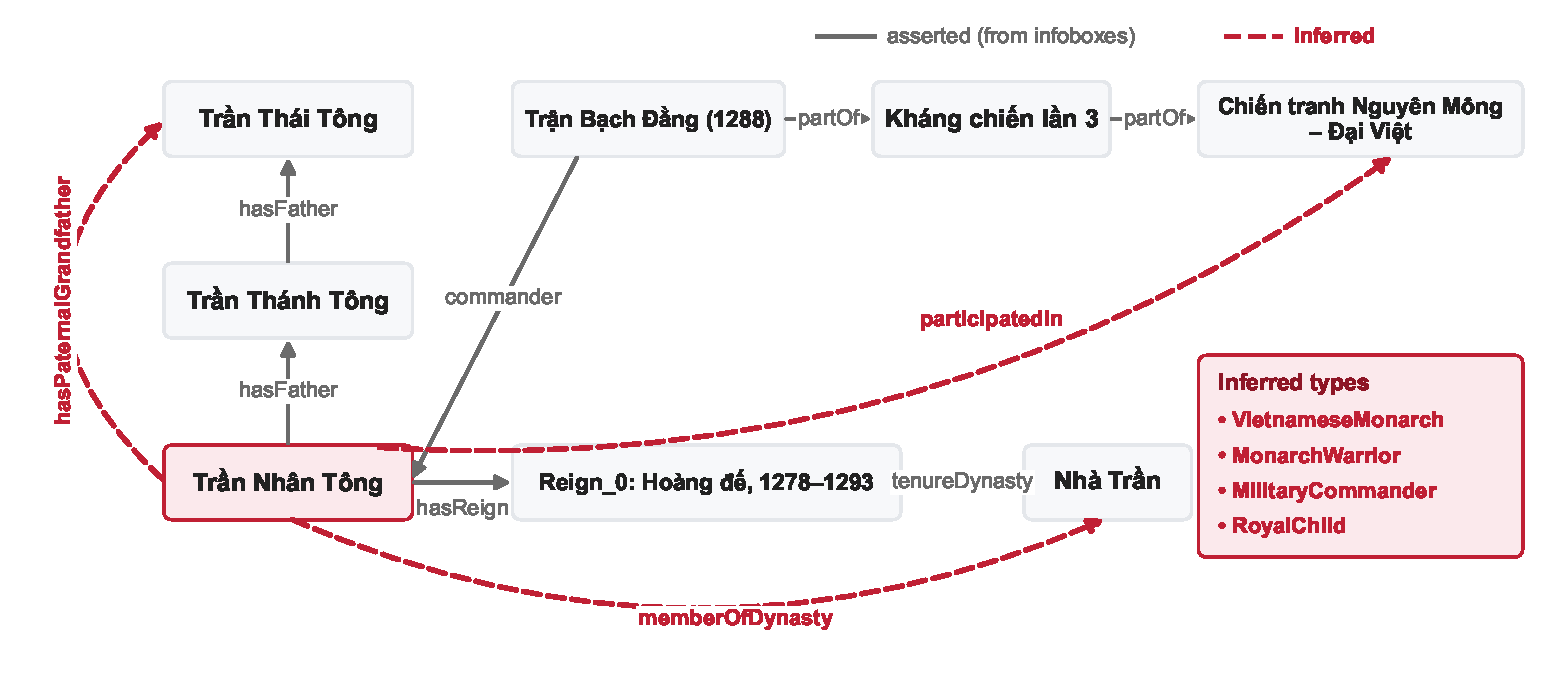
\includegraphics[width=0.68\textwidth]{figures/fig_inference.pdf}
  \caption{Asserted infobox facts (grey) and facts inferred by the ontology (red, dashed) for Trần Nhân Tông.}
  \label{fig:inference}
\end{figure}

\begin{lstlisting}[language=turtle, caption={Description of Trần Nhân Tông in ViDBpedia (excerpt), grouped by named graph.}, label=lst:sample]
# graph <.../graph/data>  (extracted from the infobox)
vidbr:Tr(*ầ*)n_Nhân_Tông a vidbo:Person, vidbo:NationalHero ;
  vidbo:hasFather vidbr:Tr(*ầ*)n_Thánh_Tông ;
  vidbo:birthPlace vidbr:Th(*ă*)ng_Long ;
  vidbo:hasReign vidbr:Tr(*ầ*)n_Nhân_Tông__Reign_0 .
# graph <.../graph/inferred>  (reasoner + rules)
vidbr:Tr(*ầ*)n_Nhân_Tông a vidbo:Monarch, vidbo:VietnameseMonarch,
    vidbo:MonarchWarrior, vidbo:RoyalChild, dbo:Person, foaf:Person ;
  vidbo:hasPaternalGrandfather vidbr:Tr(*ầ*)n_Thái_Tông ;
  vidbo:participatedIn vidbr:Chi(*ế*)n_tranh_Nguyên_Mông_(*–*)_(*Đạ*)i_Vi(*ệ*)t ;
  vidbo:bornWithin vidbr:(*Đạ*)i_Vi(*ệ*)t ;
  vidbo:sibling vidbr:Thiên_Th(*ụ*)y_Công_chúa ;     # rule R1
  vidbo:uncleOrAunt vidbr:Tr(*ầ*)n_Quang_Kh(*ả*)i ;      # chain over R1
  vidbo:ageAtDeath 50 .                           # rule R2
# graph <.../graph/links>
vidbr:Tr(*ầ*)n_Nhân_Tông owl:sameAs dbr:Tr(*ầ*)n_Nhân_Tông , wd:Q72083 .
\end{lstlisting}

\subsection{Competency questions}

All 18 CQs return answers on the local endpoint; the median execution time is 44\,ms, with a maximum of 2.1\,s for the
coverage statistics and 1.7\,s for the federated CQ13, which calls the public DBpedia endpoint. Table~\ref{tab:cq} lists
the 18 CQs with the mechanism that makes them answerable. Every CQ relies on at least one inferred triple (a defined
class, a chain, an inverse or a rule result), and CQ2 is answered entirely from the \emph{inferred} graph.
Listing~\ref{lst:cq} shows two of the formal CQs: CQ8 asks only for the inferred property \cls{bornWithin}, and CQ13 joins
local data with the public DBpedia endpoint through \ttl{owl:sameAs}.

\begin{table}[t]
  \caption{The 18 competency questions: mechanism, number of rows and execution time on the local Fuseki endpoint.}
  \label{tab:cq}
  \centering\footnotesize
  \setlength{\tabcolsep}{4pt}
  \begin{tabular}{@{}r L{4.9cm} L{6.0cm} r r@{}}
    \toprule
    CQ & Question & Mechanism (axioms / rules involved) & Rows & ms\\
    \midrule
    1 & Vietnamese monarchs by dynasty and accession year & defined classes \cls{Monarch}, \cls{VietnameseMonarch}; chain $\cls{hasReign}\circ\cls{tenureDynasty}$ & 189 & 246\\
    2 & Paternal grandfather of Trần Nhân Tông & chain $\cls{hasFather}\circ\cls{hasFather}$ & 1 & 11\\
    3 & Descendants of Trần Thái Tông & $\cls{hasParent}\sqsubseteq\cls{hasAncestor}$ (T), inverse \cls{hasDescendant} & 62 & 30\\
    4 & Vietnamese monarchs who commanded battles & $\cls{MonarchWarrior}\equiv\cls{Monarch}\sqcap\cls{MilitaryCommander}$, inverse \cls{commanded} & 89 & 47\\
    5 & Participants of the Mongol--Đại Việt war & chain $\cls{participatedIn}\circ\cls{partOfConflict}$, \cls{partOfConflict} (T) & 12 & 37\\
    6 & Reigns of the Trần dynasty with their length & n-ary \cls{Reign} nodes, rule R4 & 29 & 27\\
    7 & Conflicts per present-day province & chain $\cls{tookPlaceWithin}\circ\cls{locatedIn}$, \cls{locatedIn} (T) & 30 & 117\\
    8 & People born within today's Nghệ An & $\cls{birthPlace}\sqsubseteq\cls{bornWithin}$, chain with \cls{locatedIn} & 264 & 116\\
    9 & Provinces after the 2025 merger: communes, population, density & \cls{ThirdLevelUnit} by \texttt{hasValue}, \cls{province} $\sqsubseteq$ \cls{locatedIn}, rule R5 & 28 & 110\\
    10 & Monarchs reigning while their dynasty fought a conflict & temporal rule R6 & 166 & 30\\
    11 & Siblings, uncles/aunts and grandparents of Trần Nhân Tông & rule R1, chains \cls{uncleOrAunt}, \cls{hasGrandparent} & 20 & 34\\
    12 & People who lived to 100 or more & rules R2, R3 & 50 & 41\\
    13 & English descriptions of Lý-dynasty monarchs from DBpedia & \ttl{owl:sameAs}, SPARQL \texttt{SERVICE} & 9 & 1{,}698\\
    14 & Monarchs with the most court officials & chain $\cls{holdsOffice}\circ\cls{underMonarch}$, \cls{RoyalCourtOfficial} & 15 & 39\\
    15 & Writers influenced (directly or not) by Nguyễn Du & inverse \cls{influenced}, \cls{intellectualLineage} (T) & 2 & 10\\
    16 & Districts abolished on 1 July 2025, per province & $\cls{SecondLevelUnit}\sqsubseteq\cls{HistoricalAdministrativeUnit}$ & 65 & 48\\
    17 & Data errors (death before birth, \cls{Person} and \cls{Place}) & disjointness, comparison of years & 100 & 417\\
    18 & Share of entities linked to DBpedia, by class & \ttl{owl:sameAs} & 6 & 2{,}051\\
    \bottomrule
  \end{tabular}
\end{table}

\begin{lstlisting}[language=sparql, caption={Two formal competency questions: CQ8 (inferred property only) and CQ13 (federated with DBpedia).}, label=lst:cq]
# CQ8 - people born within today's Ngh(*ệ*) An
SELECT ?person ?label ?birthYear WHERE {
  ?person vidbo:bornWithin vidbr:Ngh(*ệ*)_An ; rdfs:label ?label .
  OPTIONAL { ?person vidbo:birthYear ?birthYear } }

# CQ13 - federated: English descriptions from DBpedia
SELECT ?label ?dbpedia ?descriptionEn WHERE {
  SERVICE <https://dbpedia.org/sparql> {
    ?dbpedia dct:subject dbc:Vietnamese_monarchs .
    OPTIONAL { ?dbpedia dbo:description ?descriptionEn
               FILTER (LANG(?descriptionEn) = "en") } }
  ?m owl:sameAs ?dbpedia ; vidbo:memberOfDynasty vidbr:Nhà_Lý ;
     a vidbo:Monarch ; rdfs:label ?label . }
\end{lstlisting}

\subsection{Verification with a tableau reasoner}

On the Trần sample, HermiT reports no unsatisfiable class and derives all eleven expected facts: the three emperors are
\cls{VietnameseMonarch}, Trần Nhân Tông is also \cls{MonarchWarrior} and \cls{RoyalChild}, Trần Hưng Đạo is
\cls{MilitaryCommander}, and the chains yield \cls{memberOfDynasty}, \cls{hasPaternalGrandfather},
\cls{participatedIn}, \cls{bornWithin} and \cls{tookPlaceWithin}. At the schema level HermiT additionally derives
$\cls{adminSeat} \sqsubseteq \cls{contains}$ from $\cls{seatOf} \sqsubseteq \cls{locatedIn}$ and the two inverse pairs,
an entailment our engine does not need because it works on the data. The same facts are produced by our RL engine on
the full data, which cross-checks the implementation.

\subsection{Data quality}\label{sec:quality}

Table~\ref{tab:quality} summarises the issues detected by the axioms and the shapes, about 1{,}700 in total. All
examples are genuine errors or ambiguities in Vietnamese Wikipedia; the article on Anna Freud, for instance, gives 1985
as her year of birth (it should be 1895), and the infobox of Lý Thái Tổ names a dynasty as his predecessor. The
transitive cycles are the largest group: most are reversed ``influenced by'' fields between writers and pairs such as
Minsk and Minsk Region, each claiming to lie within the other.

\begin{table}[t]
  \caption{Issues detected by axioms and shapes, with an example of each.}
  \label{tab:quality}
  \centering\footnotesize
  \begin{tabular}{@{}l r L{8.3cm}@{}}
    \toprule
    Check & Found & Example\\
    \midrule
    Range check at extraction & 536 & predecessor of Lý Thái Tổ = Đinh dynasty (a dynasty, not a person)\\
    Disjoint classes & 145 & a ``father'' field linking to a country ($\cls{Person} \sqcap \cls{Place} \sqsubseteq \bot$)\\
    Cycles of transitive properties & 857 & Shakespeare and Henry James influencing each other\\
    Asymmetric \cls{hasParent} & 6 & father and son swapped (Jesse Root Grant, Ulysses S. Grant)\\
    Functional \cls{birthDate} & 6 & two birth years for Alexandre de Rhodes (1591, 1593)\\
    \texttt{hasKey}(\cls{adminCode}) & 19 & 2025 communes reusing the code of a dissolved commune\\
    SHACL (closed world) & 104 & Anna Freud: born 1985, died 1982\\
    \bottomrule
  \end{tabular}
\end{table}

\subsection{Linking}

\textbf{Stage 1.} 32{,}136 of the 33{,}278 language links are verified on DBpedia (937 after a redirect); 1{,}142
point to articles missing from the DBpedia release.

\textbf{Stage 2.} On the 1{,}500-entity gold sample, the matcher reaches a precision of 96.4\% (728 correct, 27 wrong),
a recall of 48.5\% and an F1 of 0.646 at the acceptance threshold. Applied to the 10{,}930 entities without a language
link, it accepts 329 links and sends 319 candidates to review. In total ViDBpedia has 32{,}465 \ttl{owl:sameAs} links to
DBpedia and 43{,}145 to Wikidata. Table~\ref{tab:linkcls} breaks the evaluation down by class and
Figure~\ref{fig:cov} shows the resulting coverage.

\begin{table}[t]
  \caption{Stage-2 matcher on the 1,500-entity gold sample, by class.}
  \label{tab:linkcls}
  \centering\footnotesize
  \begin{tabular}{@{}l r r r r r@{}}
    \toprule
    Class & $n$ & TP & FP & Precision & Recall\\
    \midrule
    Person & 1{,}127 & 637 & 12 & 98.2\% & 56.5\%\\
    Military conflict & 126 & 0 & 0 & -- & 0.0\%\\
    State & 91 & 9 & 2 & 81.8\% & 9.9\%\\
    Place & 82 & 52 & 5 & 91.2\% & 63.4\%\\
    Administrative unit & 67 & 29 & 8 & 78.4\% & 43.3\%\\
    Other & 7 & 1 & 0 & 100\% & 14.3\%\\
    \midrule
    All & 1{,}500 & 728 & 27 & 96.4\% & 48.5\%\\
    \bottomrule
  \end{tabular}
\end{table}

\begin{figure}[t]
  \centering
  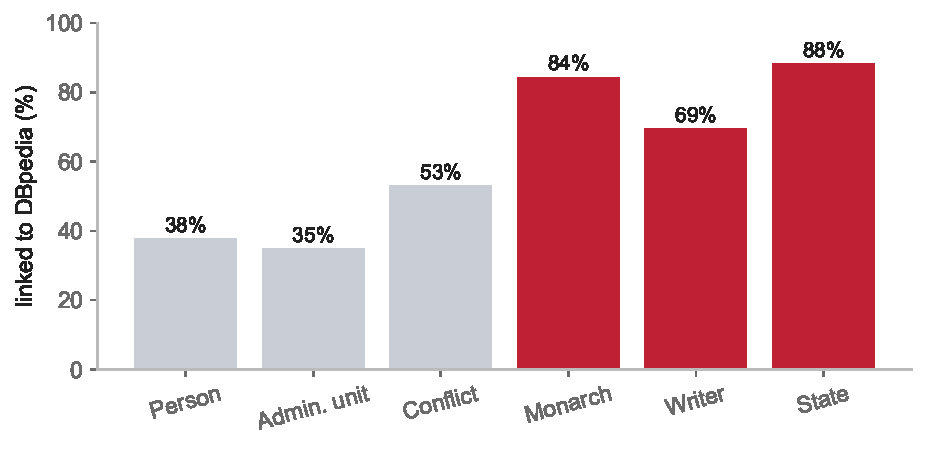
\includegraphics[width=0.44\textwidth]{figures/fig_coverage.pdf}
  \caption{Share of entities linked to English DBpedia, by class. States and monarchs are well linked; most persons
  and the new administrative units have no English counterpart.}
  \label{fig:cov}
\end{figure}

\textbf{Error analysis.} Persons, three quarters of the sample, are matched with 98.2\% precision; dates are a strong
signal for them, and the year veto removes most homonyms. Administrative units are the hardest (78.4\%): the 2025
reform created communes and wards that share names with former districts, and the matcher prefers the shorter title,
e.g.\ ``Trà Cú (huyện)'' was matched to \ttl{dbr:Trà\_Cú} instead of \ttl{dbr:Trà\_Cú\_district}. Other errors cross
types that DBpedia leaves untyped: the Vietnamese article on the destroyer \emph{USS Mannert L.\ Abele} was matched to
the person of the same name. For military conflicts the matcher proposes no candidate at all: Vietnamese battle titles
rarely translate literally into the English titles used by DBpedia, which is a limitation of label-based blocking.


\subsection{Summary of key findings}

\begin{enumerate}[leftmargin=*,itemsep=2pt]
  \item \textbf{The ontology adds more than was extracted.} Reasoning adds 2.64M triples to 627k core extracted ones;
        276k class memberships and 230k chain results are new, informative facts.
  \item \textbf{Every competency question needs inference.} All 18 CQs are answered (median 44\,ms), and none of them
        could be answered from the extracted triples alone.
  \item \textbf{Axioms double as a quality checker.} Disjointness, transitivity, functionality, keys and SHACL expose
        about 1{,}700 issues in Wikipedia, and disjointness also exposed a bug in our own extractor.
  \item \textbf{Linking is precise but incomplete.} 96.4\% precision and 48.5\% recall on 1{,}500 gold links; persons
        link well, conflicts not at all.
\end{enumerate}

% =====================================================================
\section{Discussion and Limitations}\label{sec:disc}

\textbf{Axioms are inference rules, not constraints.} The most important lesson of the project is that a domain,
range or transitivity axiom is not documentation: the reasoner applies it to every triple. Three design errors were
caught only because the reasoner amplified them. (i)~A first version declared \cls{predecessor} transitive; since
infoboxes list predecessors per office and a person holds many offices, the closure connected almost all office
holders and produced 3.8M meaningless triples. (ii)~The domain of \cls{posthumousName}, \cls{templeName} and
\cls{eraName} was \cls{Monarch}; empresses and princes also receive posthumous names, so 925 of them were inferred to be
monarchs until the domain was relaxed to \cls{Person}. (iii)~Regional infoboxes (e.g.\ the Red River Delta) list their
provinces; reading these lists as \cls{locatedIn} created containment cycles, and transitivity placed a border campaign
in a dozen provinces. CQ7 exposed the error, and the lists are now read as \cls{contains}. Because transitive properties are non-simple, OWL~2~DL cannot
declare them irreflexive; we therefore detect cycles explicitly.

\textbf{Disjointness catches software bugs.} In one run, the axiom $\cls{Person} \sqcap \cls{Tenure} \sqsubseteq \bot$
reported 17{,}841 violations. The cause was a YAML mapping key \ttl{on:} that the YAML~1.1 parser read as the boolean
\ttl{true}, which attached predecessors to tenure nodes; the domain of \cls{predecessor} then typed those nodes as
persons. No unit test would have found this: the extractor ran without error and produced plausible triples.

\textbf{Practical recommendations.} (1)~Keep the competency questions as executable queries; they decide which
axioms are worth their reasoning cost. (2)~Treat every new axiom as a code change and compare the inferred counts per
property after re-running the reasoner. (3)~Use disjointness generously: it adds no facts but is the cheapest error detector.

\textbf{Threats to validity.} The competency questions were written by us, so their success measures whether the
ontology does what we designed it to do, not how well it serves other users. The linking gold set is drawn from
entities that have an English article, which are on average better known than those without one; recall on the
entities that actually lack a link is likely lower than 48.5\%.

\textbf{Limitations and future work.} ViDBpedia covers a domain (44k of 1.6M articles) rather than the whole Vietnamese
Wikipedia; it uses a placeholder namespace (\ttl{vi.dbpedia.example.org}); lunar dates and era names are kept as
text; and stage-2 linking cannot match conflicts. Materialisation favours query speed over freshness: an update requires
re-running the reasoner. Future work includes extending the mappings to the whole Vietnamese Wikipedia, normalising
lunar dates and era names, contributing the mappings to the DBpedia community, and learning the linkage rule from the
gold pairs to improve recall.

% =====================================================================
\section{Conclusion}

ViDBpedia shows that a Vietnamese DBpedia can be more than a translation of infoboxes into RDF. An ontology designed
from competency questions, with defined classes, property chains, reified tenures and explicit knowledge about the 2025
reform, lets a simple OWL~2~RL engine add 2.64M triples to the extracted ones and answer all 18 competency questions,
while the same axioms and a set of SHACL shapes surface about 1{,}700 data-quality issues. The dataset meets the five
Linked Data stars, with 32{,}465 links to DBpedia at 96.4\% matcher precision. Beyond the specific dataset, the project
yields one transferable lesson: derive the axioms from the questions, then let the reasoner both answer the questions
and audit the data.

\textbf{Contributions of team members.} All four authors contributed equally to the project;
Table~\ref{tab:contrib} gives the per-member breakdown.

\begin{table}[t]
  \caption{Contributions of team members.}
  \label{tab:contrib}
  \centering\small
  \begin{tabular}{@{}L{2.6cm} L{5.3cm} L{5.0cm}@{}}
    \toprule
    Member & Code / module & Writing \& analysis\\
    \midrule
    Duong Hoang Hai (20252273M) & Dump collection, infobox mappings, value parsers, OWL~2~RL reasoner, rules, SHACL & \S1 Introduction; \S3 Data; \S4.2--4.4; \S6.5 Data quality\\
    Nguyen Thi Mai Anh (20252265M) & Ontology \vidbo, competency questions, HermiT verification, system demo & \S2 Related work; \S4.1 Ontology; \S6.2, \S6.4\\
    Le Phu Tai (20252268M) & DBpedia / Wikidata linking, Silk-style matcher, Fuseki endpoint, web interface, CLI & \S4.5 Interlinking; \S4.6 Publication; \S6.6 Linking\\
    Le Van Luan (20252572M) & Competency-question runner, evaluation of results and data quality & Abstract; \S5; \S6.1, 6.3, 6.7; \S7--8\\
    \bottomrule
  \end{tabular}
\end{table}

\footnotesize
\setlength{\bibsep}{0pt}
\bibliographystyle{abbrvnat}
\bibliography{references}
\normalsize

\end{document}
